%! TEX root = FIN3703_Test_2_Cheatsheet.tex
\documentclass[landscape,a4paper]{article}
\usepackage[utf8]{inputenc}
% \usepackage[T1]{fontenc}
\usepackage{tikz}
\usepackage{parskip} 
\usetikzlibrary{shapes,positioning,arrows,fit,calc,graphs,graphs.standard}
% \usepackage[nosf]{kpfonts}
% \usepackage[t1]{sourcesanspro}
\usepackage{multicol}
\usepackage{wrapfig}
\usepackage[top=5mm,bottom=5mm,left=5mm,right=5mm]{geometry}
\usepackage[framemethod=tikz]{mdframed}
% \usepackage{microtype}
\usepackage{pdfpages}
\usepackage{titlesec}
\usepackage{tabularx}
\usepackage{booktabs}
\usetikzlibrary{arrows.meta, positioning}
\usepackage[most]{tcolorbox}
\tcbuselibrary{skins,breakable}
\newtcolorbox{callout}[1][]{breakable,sharp corners, skin=enhancedmiddle jigsaw,parbox=false,
boxrule=0mm,leftrule=1mm,boxsep=0mm,arc=0mm,outer arc=0mm}

% Add these lines to create and style the column separators
\setlength{\columnseprule}{0.4pt} % Width of the rule
\setlength{\columnsep}{20pt} % Space between columns

\renewcommand{\baselinestretch}{0.5} % line spacing
\parskip=0.25pt % paragraph spacing
% \setlength\extrarowheight{5pt} % table row height
\renewcommand{\arraystretch}{1.5}
% \centering
% \titleformat*{\section}{\normalsize\bfseries}
% \titleformat*{\subsection}{\small\bfseries}

\begin{document}
%\footnotesize
% \scriptsize % 7pt
\tiny % 5pt
% \setlength{\parindent}{0pt}
\begin{multicols*}{3}
    \section{Equity Market}
\subsection{Quote Driven vs Order Driven}
Quote driven market:
\begin{itemize}
    \item Market makers provide quotes to buy/sell
    \item Market makers profit from bid-ask spread
    \item Market makers provide liquidity
    \item Market makers take on inventory risk
\end{itemize}

Order driven market:
\begin{itemize}
    \item Orders are matched by an order book
    \item No market makers
    \item No bid-ask spread
    \item No inventory risk
\end{itemize}

Limit Order Book:
\begin{itemize}
    \item Limit orders are placed in the order book
    \item Orders are matched by price, then by time
    \item A collection of not yet executed limit orders
\end{itemize}

Market Order:
\begin{itemize}
    \item Order to buy/sell at the best available price
    \item Market orders are executed immediately
    \item Certainty of execution, but no certainty of price
    \item \textbf{Consumes} liquidity
\end{itemize}

Limit Order:
\begin{itemize}
    \item Order to buy/sell at a specified price
    \item Limit orders are executed when the market price reaches the specified price
    \item Certainty of price, but no certainty of execution
    \item If the limit price crosses the threshold, it is called a \textbf{marketable limit order} and functions like a market order
    \item \textbf{Non} marketable limit orders \textbf{provide} liquidity
    \item In pure order-driven markets, limit orders are the only way to provide liquidity
\end{itemize}

\subsubsection{NYSE}
Originally a quote-driven market.
Market makers were called \textbf{specialists}.
Now a hybrid market.
\begin{itemize}
    \item \textbf{Designated Market Maker (DMM)}: Market maker that provides liquidity and maintains an orderly market
    \item \textbf{Supplemental Liquidity Providers (SLP)}: Provide liquidity by posting limit orders
    \item \textbf{Retail Liquidity Providers (RLP)}: Provide liquidity by posting limit orders
\end{itemize}

Total Market Capitalization: \$28.4 Trillion USD

\subsubsection{NASDAQ}
Originally an order-driven market. But the first electronic market with no trading floor.
Claimed to list more companies than any other exchange and has the highest trading volume. (i.e. the most liquid market)
Has multiple market makers per stock.
\begin{itemize}
    \item \textbf{Market Makers}: Provide liquidity by posting limit orders
    \item \textbf{Electronic Communication Networks (ECN)}: Facilitate trading by matching buy and sell orders
\end{itemize}

Total Market Capitalization: \$25.4 Trillion USD

\subsection{SGX}
Has multiple boards, Mainboard (Large cap), Catalist (Small cap).
Made of 2/3 local, 1/4 foreign ex-China and 1/10 China. Total listing of about 622 stocks.

Total Market Capitalization: \$811 Billion SGD

Dividends are taxed at the corporate tax rate and there is no additional dividend or withholding tax on dividends.

No foreign ownership restrictions or controls. Except for certain companies. No limit on repatriation of profits.

Clearing is done by the Central Depository (CDP).

\subsubsection{Electronic Communication Networks (ECN)}
They are alternative trading systems that allow trading outside of traditional exchanges. (Dark Pools)
They have an electronic limit order book and match buy and sell orders.
Fast execution, low cost, and anonymity.

\subsubsection{Online Brokers}
Zero comission trading.
Make money using \textbf{payment for order flow} (PFOF).
They sell their order flow to market makers who execute the trades, who then give them back a portion of the bid-ask spread.

Examples: Robinhood, E-Trade, Charles Schwab, Tiger Brokers, MooMoo.

\subsection{Behind the Scenes}
	\begin{enumerate}
		\item \textbf{Order Placement} Investor places order with broker
		\item \textbf{Order Routing} Broker sends order to market maker
			\begin{itemize}
			\item \textbf{Best Execution} Broker ensures best execution across multiple venues
		\item \textbf{Order Execution} Trade is executed at the chosen venue
			
			\end{itemize}
		\item \textbf{Trade Reporting} All trades are reported to the consolidated tape
		\item \textbf{Clearing} The National Securities Clearing Corporation (NSCC) confirms the trade details and manages the risk, reducing counterparty risk
		\item \textbf{Settlement} The Depository Trust Company (DTC) settles the trade
	\end{enumerate}

\subsubsection{Contra Trading}
Buying and selling a security before settlement, so that there is no cash outlay and only need to pay loss or receive profit. But has been on the decline due to hastening settlement cycles making this less attractive.

\subsection{Margin}
Borrowing money to buy securities and using the securities as collateral.

\textbf{Initial Margin}
The proportion of the purchase price that the investor must pay in cash.

\textbf{Maintenance Margin}
The minimum amount of equity that must be maintained in the account or else face a margin call back to this level.

\textbf{Margin Call}
When the account falls below the maintenance margin, the broker will ask the investor to deposit more money or sell some securities.

Just like in corporate finance, leverage magnifies gains and losses. But also makes things more risky.

\subsection{Short Selling}
Selling a security that you do not own, with the intention of buying it back at a lower price.

To start, borrow securities from a broker and sell them in the market.
When you buy back the securities, you return them to the broker.

The proceeds from the initial sale are not paid to the short seller, but held in the account as collateral.

Margin requirements is the normal margin requirement plus 100\% of the value of the short sale.

Equity = Original Equity + Proceeds from Short Sale $-$ Current Value of stock

Short sellers have to pay dividends to the lender of the stock.

There is limited profit potential, but unlimited loss potential. As the stock price can go up indefinitely but it can only fall to 0.

\subsection{Listing/Primary Market}
Where new securities are issued and sold to investors.

Used to raise equity for the issuer.

Initial Public Offering (IPO) is the first time a company sells its shares to the public.

Most IPOs are underwritten by investment banks and underpriced to ensure that they are fully subscribed.

Other methods of listing include:
\begin{itemize}
    \item Direct Listing: No underwriters, shares are sold directly to the public
    \item Special Purpose Acquisition Company (SPAC): A shell company that raises money through an IPO to acquire an existing company
	\item Reverse IPO: A private company acquires a public company to become public
\end{itemize}

\subsection{Delisting}
Can be voluntary or involuntary.

Voluntary delisting can be due to:
\begin{itemize}
    \item Mergers and acquisitions
    \item Going private
    \item Bankruptcy
    \item Deciding to list on another exchange
\end{itemize}

Involuntary delisting can be due to:
\begin{itemize}
    \item Not meeting listing requirements
    \item Not filing financial statements
    \item Not meeting minimum share price
    \item Bankruptcy
\end{itemize}

\subsection{Types of Shares}
\begin{itemize}
    \item \textbf{Common Shares}: Voting rights, dividends are not guaranteed
    \item \textbf{Preferred Shares}: No voting rights, dividends are guaranteed
    \item \textbf{Restricted Shares}: Shares that are subject to restrictions on resale
    \item \textbf{Treasury Shares}: Shares that have been repurchased by the company
    \item \textbf{Authorized Shares}: Maximum number of shares that a company can issue
    \item \textbf{Outstanding Shares}: Shares that are currently held by investors
\end{itemize}

\subsection{Depository Receipts}
A certificate that represents ownership of a foreign stock. It allows investors to invest in foreign companies without having to deal with foreign exchanges.

Since they are negotiable, they can be traded on local exchanges.

The foreign company's shares are purchased and placed in a custodian bank, the depository bank then issues the depository receipt to investors.

Dividends are paid in the local currency.

\subsubsection{American Depository Receipts (ADR)}
Issued in the US and denominated in USD.
A US Bank acts as the depository bank.

Often rebundled to ensure the price per ADR is attractive to investors (10-100 USD).

\subsubsection{Global Depository Receipts (GDR)}
Allows raising capital in multiple markets.
Usually one in USD and another in Europe.

\subsubsection{Singapore Depository Receipts (SDR)}
Issued in Singapore and denominated in SGD.
A Singapore bank acts as the depository bank.

Contains Thai shares.

Technically, ADRs are also able to be listed on SGX but typically see \textbf{0} volume.

\subsection{Exchange Traded Funds (ETF)}
A fund that tracks an index or a basket of assets.

They are traded on exchanges like stocks.

Value tracks the NAV of the underlying assets.

\subsubsection{Creation/Redemption Mechanism}
Authorized participants are allowed to create and redeem ETF shares. These are normally large financial institutions.
\begin{itemize}
    \item \textbf{Creation}: Authorized participants buy the underlying assets and exchange them for ETF shares
    \item \textbf{Redemption}: Authorized participants exchange ETF shares for the underlying assets
\end{itemize}

ETF Arbitrage:
\begin{itemize}
    \item If the ETF price is higher than the NAV, authorized participants will buy the underlying assets and exchange them for ETF shares
    \item If the ETF price is lower than the NAV, authorized participants will exchange ETF shares for the underlying assets
\end{itemize}

Arbitrage keeps the ETF price close to the NAV.

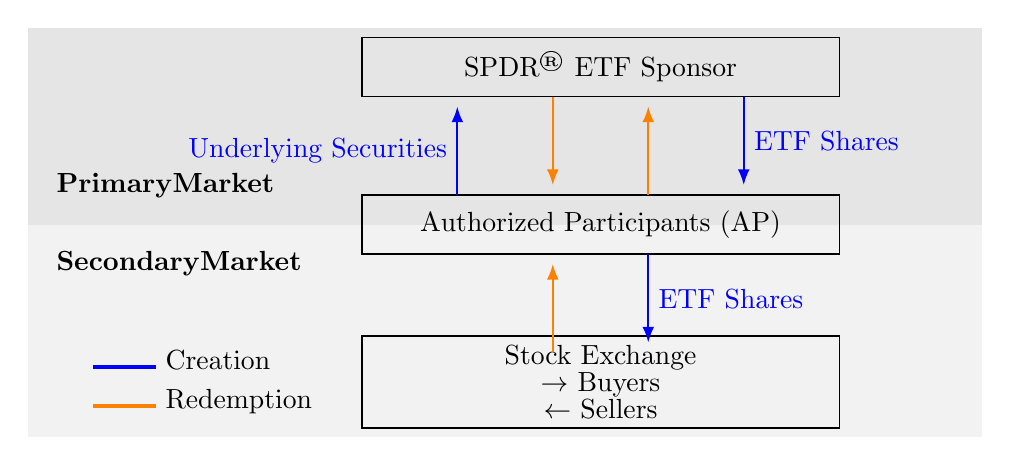
\begin{tikzpicture}[
    box/.style={draw, minimum width=0.5\columnwidth, minimum height=0.75cm, align=center, line width=0.5pt},
    arrow/.style={-{Latex[length=2mm]}, thick},
    creation/.style={arrow, blue},
    redemption/.style={arrow, orange}
]

% Background rectangles for markets with relative positioning
\fill[gray!20] (-0.1\columnwidth,-0.5) rectangle (0.9\columnwidth,3);
\node[anchor=west] at (-0.08\columnwidth,1) {\textbf{Primary}\\\textbf{Market}};

\fill[gray!10] (-0.1\columnwidth,0.5) rectangle (0.9\columnwidth,-2.2);
\node[anchor=west] at (-0.08\columnwidth,0) {\textbf{Secondary}\\\textbf{Market}};

% Boxes
\node[box] (sponsor) at (0.5\columnwidth,2.5) {SPDR\textsuperscript{\textregistered} ETF Sponsor};
\node[box] (ap) at (0.5\columnwidth,0.5) {Authorized Participants (AP)};
\node[box] (exchange) at (0.5\columnwidth,-1.5) {Stock Exchange \\ {$\rightarrow$ Buyers} \\ {$\leftarrow$ Sellers}};

% Vertical arrows and labels between sponsor and AP
\draw[creation] (0.35\columnwidth,0.88) -- (0.35\columnwidth,2) node[midway, left, blue] {Underlying Securities};
\draw[redemption] (0.45\columnwidth,2.12) -- (0.45\columnwidth,1);
\draw[creation] (0.65\columnwidth,2.12) -- (0.65\columnwidth,1) node[midway, right, blue] {ETF Shares};
\draw[redemption] (0.55\columnwidth,0.88) -- (0.55\columnwidth,2);

% Vertical arrows and labels between AP and exchange
\draw[creation] (0.55\columnwidth,0.12) -- (0.55\columnwidth,-1) node[midway, right, blue] {ETF Shares};
\draw[redemption] (0.45\columnwidth,-1.12) -- (0.45\columnwidth,0);

% Legend
\node[left=0.5cm of exchange, align=left] (legend) {
    \textcolor{blue}{\rule{0.8cm}{1.5pt}} Creation \\
    \\
    \textcolor{orange}{\rule{0.8cm}{1.5pt}} Redemption
};

\end{tikzpicture}


\subsection{REITs}
Real Estate Investment Trusts are companies that own, operate, or finance income-producing real estate.

REITs allow investors to invest in real estate without having to buy property.

Started in the US as a pass-through entity, meaning that they do not pay corporate tax if they distribute 90\% of their income to shareholders.

REITs are required to distribute 90\% of their income to shareholders.

In Singapore, REITs are allowed to invest in other assets but the majority of their income must come from real estate.

Also granted tax transparency if they distribute 90\% of their income in Singapore.



\end{multicols*}


\end{document}
